\chapter{Draft}

\section{RQ1. Com que frequência \textit{breaking changes} surgem nos pacotes clientes?}
\label{sec:rq1}

\subsection{Motivação}
\label{mot:rq1}

No ecossistema do \gls{NPM}, uma simples \textit{release} que contenha um erro pode afetar uma quantidade imensa de pacotes, uma vez que este repositório contém a maior rede de dependências entre pacotes \cite{teorical_reference:npm_2}. Para evitar que \textit{breaking changes} se manifestem nos pacotes clientes, os provedores introduzem as \textit{breaking changes} em \textit{releases major}, seguindo o padrão do Versionamento Semântico, e os cliente podem utilizar \textit{strings semver} para aceitar apenas as versões \textit{minor} e \textit{patch} dos provedores -- o que é o padrão do \gls{NPM}. Entretanto, nem sempre o provedor é capaz de distinguir se suas alterações são \textit{breaking} ou \textit{non-breaking changes} \cite{noregrets2018}, ou, muitas vezes, as \textit{breaking changes} são introduzidas sem que o provedores percebam. Portanto, quando as \textit{breaking changes} são introduzidas em \textit{releases minor} ou \textit{patch}, elas podem causar comportamentos inesperados no cliente. Nesta RQ, será quantificado as manifestações das \textit{breaking changes} nos pacotes clientes. Assim, entender a frequência que os provedores publicam \textit{breaking changes} que afetam os clientes pode ajudar os clientes a fazer decisões melhores sobre como e quando atualizar a versão do seu provedor.

\subsection{Método}
\label{apr:rq1}

%\Gls{NPM}.
Um \textit{stack trace} é utilizado pelo \gls{NPM} para apresentar informações sobre um determinado erro. Quando os comandos \textit{npm install} e \textit{npm test} resultam em erro, o \Gls{NPM} mostra o erro e todas as chamadas de funções, incluindo as invocações para os provedores. A Figura \ref{fig:trace} mostra um exemplo genérico de um \textit{stack trace} exibido pelo \Gls{NPM}. Nesta Figura, no topo do \textit{stack trace}, contém o tipo do erro que interrompeu a execução e a sua mensagem. Nas linhas abaixo, há todas as funções e arquivos que foram executados até a manifestação do erro. Com todos estes dados, o \textit{stack trace} auxiliou no rastreamento de cada erro, uma vez que ele foi utilizado para detectar as \textit{breaking changes}, pois através do \textit{stack trace} foi possível identificar com exatidão em qual pacote o erro se manifestou: no ciente ou no provedor.

\begin{figure}
    \centering
    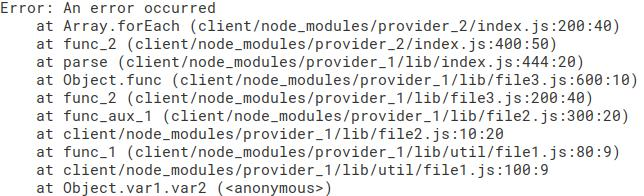
\includegraphics[scale=0.7]{figuras/stack_trace.jpeg}
    \caption{\textit{stack-trace} genérico}
    \label{fig:trace}
\end{figure}{}

Para quantificar as \textit{breaking changes}, foi necessário diferenciar entre um erro que foi causado pelo próprio pacote cliente, no qual não houve influência de nenhum provedor, e um erro que foi causado por algum dos provedores, sendo assim uma \textit{breaking change}. Esta diferenciação é necessária pois um determinado erro pode ter ocorrido no código do cliente e não em um provedor, assim não sendo um caso de \textit{breaking change}. Para realizar esta diferenciação, foi utilizado as seguintes heurísticas:

\begin{itemize}
    \item Verificar no \textit{stack trace}:
    \begin{itemize}
        \item quando não houve registros de execução dos provedores no \textit{stack trace}, provavelmente o erro não foi causado por uma \textit{breaking change}. Assim, o erro podia estar apenas no código do cliente; e

        \item quando houve registros de execução dos provedores no \textit{stack trace}, o erro provavelmente se tratava de uma \textit{breaking change}. Entretanto, as chamadas para \textit{frameworks} de teste, como o \textit{Mocha\footnote{https://www.npmjs.com/package/mocha}, Jasmine\footnote{https://www.npmjs.com/package/jasmine}} entre outros, ou automatizadores de tarefas, como o \textit{Grunt\footnote{https://www.npmjs.com/package/grunt}} por exemplo, não evidenciavam, inicialmente, a presença de \textit{breaking changes} uma vez que eles apenas iniciam a execução do pacote. Porém, não foi descartada a hipótese deles apresentarem \textit{breaking changes}.
    \end{itemize}{}

    \item  Próximos \textit{commits} do cliente: foi verificado no \textit{GitHub} se o cliente tentou consertar algum erro após a \textit{release} que apresentou o erro. Se foi encontrado algum \textit{commit} com correções, foram feitas estas alterações no código do cliente para verificar se as modificações encontradas no \textit{GitHub} realmente refletiam a correção do erro. Assim, se as alterações apenas no código do cliente refletiam na correção do erro, sem que haja influência dos provedores, então o erro não se tratava de uma \textit{breaking change};

    \item Sistemas integrados ao \textit{GitHub}: alguns sistemas integrados ao \textit{GitHub} auxiliaram na investigação. Esses sistemas são o \textit{Travis\footnote{https://travis-ci.org}, Codeship\footnote{https://codeship.com}} entre outros, que armazenam os resultados da execução do pacote para cada \textit{commit}. Eles foram utilizados da seguinte maneira: se nesses sistemas integrados, a execução no \textit{commit} da \textit{release} do cliente foi realizado com sucesso e, ao executá-lo nesta pesquisa, resultou em erro, significa que houve uma \textit{breaking change}, uma vez que o código do cliente estava na mesma \textit{working tree} do \textit{commit}. Mas, se a execução do cliente no momento do \textit{commit} resultou em erro, provavelmente os próximos \textit{commits} contêm alguma informação sobre o erro e sua correção, uma vez que estes sistemas integrados avisaram os desenvolvedores sobre o erro na execução.
\end{itemize}{}

Portanto, cada erro foi analisado manualmente, com alterações no código do cliente, para certificar se o erro era uma \textit{non-break change} ou uma \textit{break change}. Essa separação foi importante para esta e para as próximas questões de pesquisa. Com isto, foi quantificado os casos \textit{breaking changes} por \textit{releases}.

\subsection{Resultados}
\label{fin:rq1}
Ao todo, 384 pacotes foram utilizados nesta pesquisa e foram executadas pelo menos uma de suas \textit{releases}. Desses 384 pacotes, 244 resultaram em falhas para alguma de suas \textit{releases}. Já analisando as \textit{releases}, de todas as 4570, foram executadas um total de 2662 \textit{releases}, pois possuíam adições ou alterações em suas dependências e estavam passíveis de sofrerem com \textit{breaking change}. Após a execução, 1460 


\textit{releases} resultaram em erro no \textit{script install} ou \textit{test}, e foram analisadas manualmente. Por fim, 1908 \textit{releases} não foram executadas pois não haviam alterações nas \textit{releases} dos provedores, mas apenas alterações no código do cliente, o que não tem possibilidade da manifestação de uma \textit{breaking changes}. A Figura \ref{fig:result_rq1_g} apresenta esses resultados, no qual o gráfico externo apresenta a proporção de sucesso e de erro por pacotes e por \textit{releases} no gráfico interno.

\begin{figure}
    \centering
    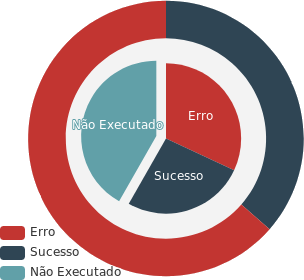
\includegraphics[scale=0.8]{figuras/result_rq1_g.png}
    \caption{Proporção de sucesso e erro da execução: por pacote -- gráfico externo -- e por \textit{releases} -- gráfico interno}
    \label{fig:result_rq1_g}
\end{figure}{}

\subsubsection{De todos os pacotes, 11\% foram impactados por \textit{breaking changes}}
Após a análise manual em cada uma das \textit{releases} que resultaram em erro, foi constatado um total de 11\% de pacotes que foram impactados por \textit{breaking changes}.



\subsubsection{Dos pacotes afetados, 13\% apresentaram mais de uma \textit{breaking change}}

\subsubsection{22\% das \textit{breaking changes} foram causadas por provedores indiretos}

\subsubsection{Os maiores provedores causaram mais \textit{breaking changes}}

%---------------------------------------------------%
\section{RQ2. Como os pacotes provedores introduzem \textit{breaking changes} em uma \textit{release}?}
\label{sec:rq2}

\subsection{Motivação}
\label{mot:rq2}
Pesquisas anteriores apresentam estudos sobre \textit{breaking changes} no ecossistema do \gls{NPM}. Entretanto, pelo fato do \textit{Javascript} ser dinâmico, estes estudos focaram apenas nas alterações de \gls{API}, tais como as remoções/renomeações, alterações na lista de parâmetros e alterações no tipo de retorno. Estes estudos foram realizados por  \citeonline{teorical_reference:bc_1} e \citeonline{noregrets2018} e não verificaram \textit{breaking changes} além das relacionadas às \gls{API}. Desta maneira, além das alterações em \gls{API}, não se tem informações sobre como os provedores introduzem \textit{breaking changes}, ou seja, quais os principais casos que fazem com que o cliente sofra uma \textit{breaking changes}. Por causa da falta de informação, muitas \textit{breaking changes} são introduzidas, mas poderiam ser facilmente evitadas. Assim, grande parte das \textit{breaking changes} em \textit{JavaScript} são detectadas apenas em tempo de execução \cite{noregrets2018}, mas para o cliente, ter seu código encerrado em tempo de execução pode ser muito custoso. Por isso, dimensionar e categorizar as \textit{breaking changes} ajudará os desenvolvedores a atentar-se para as \textit{breaking changes} mais comuns e tentar evitá-las, assim produzindo códigos menos favoráveis às \textit{breaking changes}.

\subsection{Método}
\label{apr:rq2}
O objetivo da análise manual é descobrir o motivo que originou uma \textit{breaking changes}, ou seja, qual foi a alteração que o provedor realizou que causou a \textit{breaking change}, para que seja possível agrupa-las por suas similaridades. Porque o \textit{stack trace} sempre apresenta o erro de uma maneira genérica, às vezes, a mensagem de erro pode induzir a interpretação errônea do real motivo que originou a falha. Assim, o melhor local para se investigar quais foram as alterações que o provedor realizou é o \textit{GitHub}, no qual várias técnicas foram utilizadas para recuperar as informações necessárias:

\begin{itemize}
    \item Arquivos de alterações: os arquivos de registros de alterações, comumente nomeados por \textit{CHANGELOG.md} ou \textit{HISTORY.md}, contêm as descrições das principais alterações em cada \textit{releases} do projeto. Através da versão do provedor que foi descarregada do \gls{NPM}, foi verificado nos arquivos de alterações quais foram as modificações introduzidas pelos provedores e se alguma destas alterações diz respeito ao erro encontrado no cliente. Uma das informações mais relevantes nestes arquivos são as descrições de \textit{breaking changes}. Por exemplo, a versão \textit{5.0.0} do pacote \textit{Mocha} contém uma \textit{breaking change} que foi documentada no \textit{CHANGELOG.md}\footnote{https://github.com/mochajs/mocha/blob/master/CHANGELOG.md\#500--2018-01-17} de acordo com a Figura \ref{fig:bc_documentation} (a). Outro tipo de documentação equivalente são as \textit{releases-notes}, como pode ser visualizado na Figura \ref{fig:bc_documentation} (b) como o pacote \textit{wpxml2md} documentou \textit{breaking changes} nas \textit{releases-notes}\footnote{https://github.com/akabekobeko/npm-wpxml2md/releases/tag/v2.0.0}. Entretanto, apenas 46\% dos repositórios utilizados nesta pesquisa contêm algum dos dois registros.

    \item \textit{Issues/Pull-requests}: uma vez que uma \textit{breaking change} se manifesta em algum cliente, ele pode -- e deve -- registrar este erro através de uma \textit{issue} no repositório do provedor. O proveito de buscar informações nas \textit{issues} é que essas contêm comentários dos provedores e da comunidade, assim, há muitas informações sobre um determinado erro, além de várias outras \textit{issues} lincadas, ampliando a busca por informações. Da mesma maneira os \textit{pull-requests} foram utilizados para buscar informações sobre as \textit{breaking changes}.

    \item Versões prévias dos provedores: um ponto muito importante foi a instalação de versões prévias dos provedores. Uma vez que foi identificado qual provedor está causando a \textit{breaking change}, a instalação de outras versões ajudaram a descobrir a partir de qual \textit{release} do provedor a \textit{breaking change} foi introduzida, ou a partir de qual \textit{release} ela foi consertada. Com isso, as \textit{breaking change} ficaram mais fáceis de serem identificadas pois, uma vez que foi localizada a \textit{release} que introduziu o erro, pode ser utilizado ferramentas de \textit{diff} para analisar o código introduzido e removido daquela \textit{release}.

    \item Ferramentas de \textit{diff}: o uso da ferramenta que realizam o  \textit{diff} entre duas \textit{releases} de um pacote foi muito importante. Foi utilizado a ferramenta \textit{npm-diff}\footnote{https://github.com/danielventurini/npm-diff} e a ferramenta \textit{compare}\footnote{https://github.com/danielventurini/cnlg/compare/1.1.0..1.1.1} do \textit{GitHub}. Com isso, foi possível verificar o que foi adicionado e removido do código do provedor -- até mesmo do cliente -- em um determinado intervalo de versões.
\end{itemize}

\begin{figure}
    \centering
    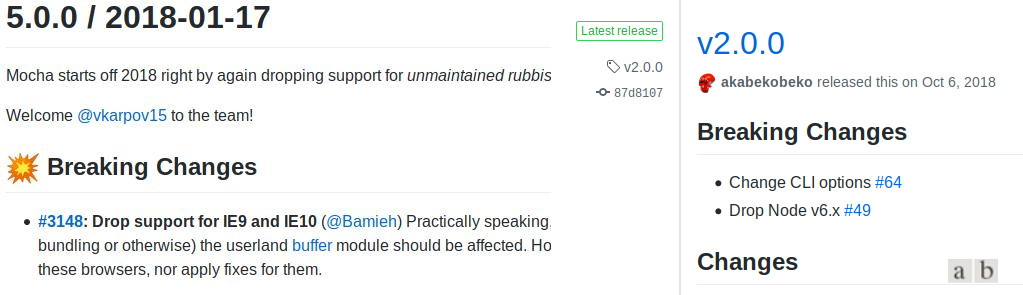
\includegraphics[scale=0.45]{figuras/bc_documentation.jpeg}
    \caption{Documentação de uma \textit{breaking change} no \textit{CHANGELOG} e nas \textit{release-notes}}
    \label{fig:bc_documentation}
\end{figure}{}

Após descobrir que o de alteração que introduziu uma \textit{breaking change}, categorias foram criadas para agrupar as \textit{breaking changes}. Por exemplo, quando um erro tratava-se de uma alteração de \gls{API}, uma categoria chamada \textit{Função Renomeada} foi criada e as demais \textit{breaking changes} que possuem características comuns a esta também foram categorizadas como \textit{Função Renomeada}. Assim será possível quantificar cada uma das categorias e visualizar as mais comuns. E o mesmo processo foi realizado para as demais \textit{breaking changes}, sempre visando criar categorias da maneira mais genérica que agrupassem os erros semelhantes.

Então, para todas as \textit{releases} analisadas manualmente, foram salvas as seguintes informações para que fosse possível quantificar as \textit{breaking changes} e responder esta e as demais questões de pesquisas:

\begin{enumerate}
    \item Em que local o erro foi documentado: \textit{issue, changelog, pull-request} etc;
    \item Quem consertou o erro: cliente ou providor;
    \item Em qual nível do \textit{SEMVER} o erro foi reparado;
    \item Quanto tempo o erro levou até ser corrigido; e
    \item Por quantas \textit{releases} o erro persistiu.
\end{enumerate}{}


\subsection{Resultados}
\label{fin:rq2}

%---------------------------------------------------%
\section{RQ3. Como os pacotes clientes se recuperam das \textit{breaking changes}?}
\label{sec:rq3}

\subsection{Motivação}
\label{mot:rq3}
Uma vez que uma \textit{breaking changes} é introduzida, o cliente deve se recuperar dessa, ajustando o seu próprio código. Isso se faz necessário pois, no ecossistema do  \gls{NPM}, no qual centenas de milhares de pacotes estão conectados, uma simples \textit{release} com erro pode ocasionar na quebra de muitos clientes. No entanto, como os provedores evoluem independentemente dos clientes, erros e vulnerabilidades são difíceis de rastrear e corrigir nos clientes. Mesmo quando as vulnerabilidades podem ser corrigidas com a atualização para uma versão mais recente do provedor, pode haver incompatibilidades de \textit{API} -- entre outras incompatibilidades -- com os clientes que deve ser resolvido manualmente \cite{Foo:2018:ESC:3236024.3275535}. Desta maneira, entender como o cliente reagem às \textit{breaking changes} ajudará os clientes a conhecerem as alternativas frente às \textit{breaking changes} para que eles possam se recuperar da maneira mais eficiente.

\subsection{Método}
\label{apr:rq3}
Uma vez que os clientes se recuperaram de um erro, há duas maneiras para se obter informações sobre esta recuperação. A primeira maneira é quando o provedor corrige seu código e o cliente apenas atualiza sua \textit{string} de versionamento no \textit{package.json}. Para o provedor consertar o erro, deve haver uma \textit{issue} no seu repositório. A segunda maneira é quando o próprio cliente conserta o código. Neste caso, o cliente pode corrigir o código do provedor e realizar um \textit{pull-request}. Também, o cliente pode alterar apenas o seu código para que execute normalmente com a \textit{release} do provedor que introduziu a \textit{breaking change}.

Todas as informações sobre esta questão de pesquisa foram recuperadas do \textit{GitHub}. As informações foram encontradas em \textit{CHANGELOGs, release-notes, issues} e \textit{pull-requests}. Os \textit{CHANGELOGs} contêm informações sobre os erros consertados. A partir das \textit{issues} é possível entender com os comentários dos clientes quais foram as ações que eles realizaram para se recuperar de uma determinada \textit{breaking change}. Pois, assim como o código de um pacote fica emaranhado com o código no restante do ecossistema ao qual ele pertence, o mesmo acontece com as \textit{issues}. Uma manifestação disso é que muitas \textit{issues} abertas em um projeto são vinculadas a \textit{issues} relacionadas, em projetos iguais ou diferentes, pois os desenvolvedores estão rastreando as causas de um problema \cite{Zhang:2018:WIL:3242887.3242891}. De maneira análoga, os \textit{pull-requests} que são relacionados ao mesmo problema também são marcados. Todas estas informações corroboram para descobrir como a \textit{breaking change} foi tratada/consertada e quem -- cliente ou provedor -- a consertou, caso tenha sido consertada.

Os \textit{commits} são alternativas para as \textit{issues} quando a busca se dá no repositório do cliente. Sobre os \textit{commits}, mensagens do tipo \textit{update dependencies, fix dependencies, fix errors} etc. sugerem que algum provedor foi atualizado para consertar algum erro ou um erro foi consertado diretamente no código do cliente. Estas informações são muito importantes, uma vez que o provedor corrigiu a \textit{breaking change} e o cliente apenas o atualizou. Assim, as mensagens dos \textit{commits} auxiliaram para descobrir os reais motivos da atualização -- ou retrocesso da versão.

\subsection{Resultados}
\label{d_fin:rq3}



